\chapter{Gap-Filling} \label{Chap4}

\section{Overview}

Chapter~\ref{Chap3} showed that raw hourly FCH\textsubscript{4} was unavailable
for 86.8\%, 50.3\% and 71.5\% of the common analysis window at T2, T4 and T9,
respectively. After applying the target quality and plausibility criteria,
effective unavailability increased to 92.0\%, 68.3\% and 81.7\%
(Table~\ref{tab:ch3_fch4_missingness}). Chapter~\ref{Chap3} reconstructed the
supporting environmental variables to provide a complete predictor frame but
deliberately left FCH\textsubscript{4} unfilled. Reconstructing this remaining
target supports continuous retrospective analysis and downstream model
configurations that require an uninterrupted methane history.

The experiments use the tower-specific hourly modelling frames constructed in
Chapter~\ref{Chap3}. The response variable is QC-valid observed
FCH\textsubscript{4}, while the expanded predictor frame combines current
environmental conditions, carbon-cycle variables, calendar encodings,
livestock information, environmental history and management events.
Table~\ref{tab:gf_features} summarises these inputs.

\begin{table}[htbp]
\centering
\small
\renewcommand{\arraystretch}{1.15}
\caption{Expanded predictor frame used in the gap-filling benchmark. Counts
exclude the FCH\textsubscript{4} target and tower-indicator variables.}
\label{tab:gf_features}
\begin{tabular*}{\textwidth}{@{\extracolsep{\fill}}
>{\raggedright\arraybackslash}p{0.22\textwidth}
>{\raggedright\arraybackslash}p{0.63\textwidth}
>{\centering\arraybackslash}p{0.07\textwidth}@{}}
\toprule
Feature group & Variables & Count \\
\midrule
Current environmental conditions &
SWIN, TA, VPD, PPFD, RN, WS, USTAR, SHF, precipitation,
soil temperature and soil moisture &
11 \\
\addlinespace[0.35em]

Carbon cycle &
Gap-filled FCO\textsubscript{2}, GPP and ecosystem respiration &
3 \\
\addlinespace[0.35em]

Calendar &
Cyclic hour-of-day and day-of-year sine and cosine encodings &
4 \\
\addlinespace[0.35em]

Livestock &
Livestock-unit density and grazing-presence indicator &
2 \\
\addlinespace[0.35em]

Environmental history &
Soil-moisture and soil-temperature lags at 168, 336, 504 and
672 hours &
8 \\
\addlinespace[0.35em]

Management &
Recency of cutting and manure application &
2 \\
\midrule
\textbf{Total} & & \textbf{30} \\
\bottomrule
\end{tabular*}
\end{table}

The expanded 30-predictor frame was used for the principal tabular benchmark.
Models sharing data across towers additionally received three tower-indicator
variables, whereas TabICLv2 did not require them.
MDS used only shortwave radiation, air temperature and VPD, while the
meteorology-only Random Forest used the 11 current environmental variables.
SAITS and Bi-LSTM omitted the eight explicit soil-lag variables because
temporal context was supplied directly through their input sequences.
Published-baseline replications retained their corresponding study-specific
feature subsets.

All models were evaluated using the synthetic-gap protocol defined in
Chapter~\ref{ChapModels}. Consequently, the reported scores measure recovery
of deliberately masked observations for which ground truth exists; they do not
establish that predictions made during naturally unobserved intervals are
equivalent to measurements. The following sections compare the complete model
roster against literature-aligned baselines and evaluate prediction-interval
calibration.

\FloatBarrier

\section{Results}

Unless otherwise stated, results are the median tower-specific \(R^2\) values,
calculated using the OLS convention defined in Chapter~\ref{ChapModels}, under
the common synthetic-gap protocol. Combined results are equal-weight
averages over T2, T4 and T9, preventing the longer T4 record from
dominating the comparison. Because this form of \(R^2\) measures linear
agreement rather than absolute calibration, the accompanying uncertainty
analysis is used to qualify the headline ranking.

\subsection{Full Model Comparison}

MDS and the meteorology-only Random Forest provide literature-aligned reference
points within the common benchmark, with Zhu et al. serving as the closest
same-site comparator \cite{zhu2023a}. Adaptations of the broader Irvin and Kim
benchmarks are retained in Appendix Table~\ref{tab:gf_published_replication} for
context rather than treated as controlled cross-study comparisons.

\begin{table}[htbp]
\centering
\footnotesize
\begin{tabular*}{\textwidth}{@{\extracolsep{\fill}}lrrrrr@{}}
\toprule
Model or experiment & T2 $R^2$ & T4 $R^2$ & T9 $R^2$ & Combined & \shortstack{Improvement\\over MDS} \\
\midrule
Training-set mean & -- & -- & -- & -- & -- \\
MDS & 0.072 & 0.038 & 0.054 & 0.055 & 0.000 \\
RF (meteorology features only) & 0.054 & 0.042 & 0.065 & 0.054 & $-0.001$ \\
MICE & 0.104 & 0.128 & 0.110 & 0.114 & $+0.059$ \\
HyperImpute & 0.567 & 0.352 & 0.362 & 0.427 & $+0.372$ \\
RF (additional features) & 0.601 & 0.409 & 0.430 & 0.480 & $+0.425$ \\
LightGBM & 0.583 & 0.418 & 0.425 & 0.475 & $+0.420$ \\
XGBoost & 0.619 & 0.380 & 0.375 & 0.458 & $+0.403$ \\
SAITS & 0.562 & 0.289 & 0.304 & 0.385 & $+0.330$ \\
Bidirectional LSTM & 0.280 & 0.204 & 0.189 & 0.224 & $+0.169$ \\
\textbf{TabICLv2} & \textbf{0.686} & \textbf{0.429} & \textbf{0.430} & \textbf{0.515} & $\mathbf{+0.460}$ \\
\bottomrule
\end{tabular*}
\caption{Full gap-filling model comparison under the common synthetic-gap
protocol. Combined values are equal-weight averages of the three
tower-specific \(R^2\) scores; improvement over MDS is the difference between
each model's combined score and the combined MDS score. The training-set mean
is constant, so its squared-correlation \(R^2\) is undefined.}
\label{tab:gf_model_comparison}
\end{table}

Table~\ref{tab:gf_model_comparison} shows that TabICLv2 produced the strongest
overall linear agreement, leading at T2 and T4, matching the expanded Random
Forest at T9, and attaining a combined \(R^2\) of 0.515. The
expanded Random Forest and LightGBM remained close at 0.480 and 0.475,
respectively, whereas MICE and the two deep sequence models were weaker. The
results therefore do not support a general claim that deep learning is
superior to traditional machine learning: performance depended on the model
architecture and its use of the available context. TabICLv2 is therefore
retained as the gap-filling champion.
Aggregate MAE and RMSE values for the same model comparison are reported in
Appendix Table~\ref{tab:gf_error_metrics_aggregate}.

Relative to MDS, the combined \(R^2\) increased by 0.425 for the expanded
Random Forest and 0.460 for TabICLv2; their tower-specific gains ranged from
0.371 to 0.614. These are reported as additive changes rather than percentage
gains because ratios against an \(R^2\) value close to zero would exaggerate
the apparent improvement.

\begin{figure}[htbp]
\centering
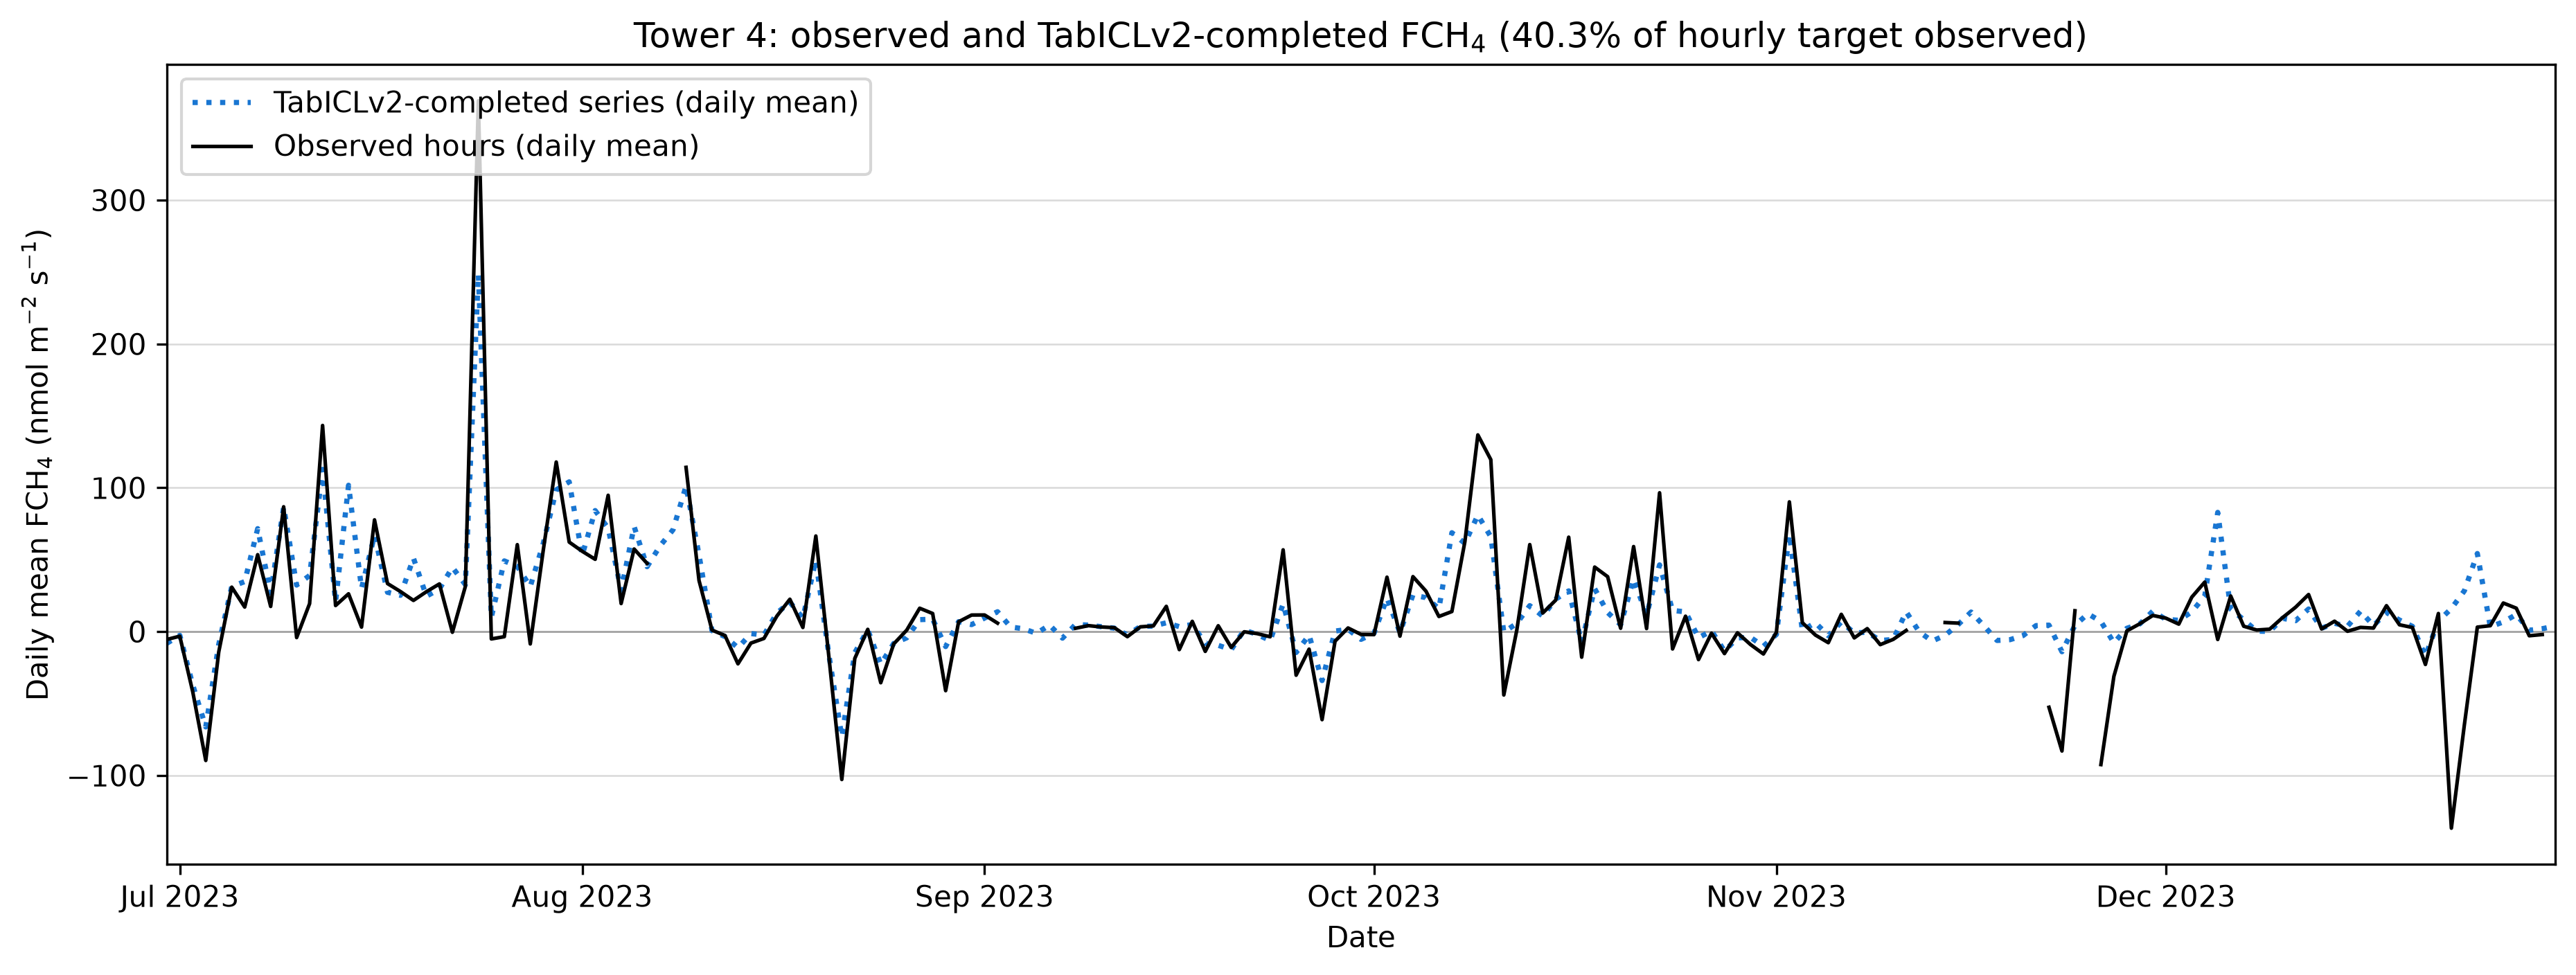
\includegraphics[width=\textwidth]{Figures/ch4_tabiclv2_daily_T4_2023H2.png}
\caption{Daily means of QC-valid observed hours (solid black) and the
TabICLv2-completed series (dotted blue) at T4 from July to December 2023, when
40.3\% of the hourly FCH\textsubscript{4} target was observed. The completed
series preserves observations and replaces missing hours with TabICLv2
estimates; the comparison is therefore a reconstruction diagnostic rather
than held-out validation. Corresponding T2 and T9 reconstructions are provided
in Appendix Figure~\ref{fig:app_gf_tabicl_daily_t2_t9}.}
\label{fig:gf_t4_reconstruction}
\end{figure}

Figure~\ref{fig:gf_t4_reconstruction} illustrates the operational effect of
applying TabICLv2 to a sparse measurement period. The completed series
provides a continuous daily trajectory and follows the broad observed
variation, although several peaks are attenuated. Its overlap with the
observed line is expected because measured hours are preserved rather than
replaced. The figure therefore demonstrates the operational reconstruction
while retaining the distinction between estimates and direct measurements.

\FloatBarrier

\subsection{Uncertainty Quantification} \label{gf:uq}
Raw 90\% prediction intervals were obtained from Quantile Regression Forests
for RFm and native quantile predictions for TabICLv2. Split-conformal
calibration was then evaluated separately within each tower and gap-duration
setting, following Chapter~\ref{ChapModels}.

\begin{table}[htbp]
\centering
\footnotesize
\begin{tabular*}{\textwidth}{@{\extracolsep{\fill}}llrrrrr@{}}
\toprule
Model & Tower & $n$ & \shortstack{Raw\\PICP} & \shortstack{Calibrated\\PICP} & \shortstack{Raw\\MPIW} & \shortstack{Calibrated\\MPIW} \\
\midrule
QRF (additional features) & T2 & 4,961 & 0.938 & 0.893 & 163.8 & 147.6 \\
 & T4 & 19,485 & 0.917 & 0.901 & 196.1 & 186.8 \\
 & T9 & 11,279 & 0.902 & 0.903 & 214.2 & 216.2 \\
 & \textbf{Average} & \textbf{35,725} & \textbf{0.919} & \textbf{0.899} & \textbf{191.4} & \textbf{183.5} \\
\addlinespace[0.3em]
TabICLv2 (quantile) & T2 & 4,961 & 0.918 & 0.904 & 134.5 & 130.1 \\
 & T4 & 19,485 & 0.899 & 0.899 & 181.6 & 181.2 \\
 & T9 & 11,279 & 0.888 & 0.893 & 214.5 & 217.2 \\
 & \textbf{Average} & \textbf{35,725} & \textbf{0.902} & \textbf{0.899} & \textbf{176.8} & \textbf{176.2} \\
\bottomrule
\end{tabular*}
\caption{Raw and split-conformal 90\% prediction-interval performance on the
held-out calibration-test subset of the synthetic-gap experiment. PICP has a
nominal target of 0.90; MPIW is reported in
\(\mathrm{nmol\,m^{-2}\,s^{-1}}\). Tower rows are equal-weight means across
the four gap-duration settings; averages weight all tower--gap cells
equally, while \(n\) reports their total test observations.}
\label{tab:gf_uq_calibration}
\end{table}

\FloatBarrier

Both raw interval methods were close to the 0.90 nominal target
(Table~\ref{tab:gf_uq_calibration}). Calibration reduced average QRF
coverage from 0.919 to 0.899 while narrowing MPIW from 191.4 to 183.5.
TabICLv2 moved from 0.902 to 0.899 coverage while MPIW changed only from 176.8
to 176.2. Across the
individual tower--gap cells, calibrated coverage ranged from 0.876 to 0.912
for QRF and from 0.888 to 0.910 for TabICLv2. Figure~\ref{fig:gf_tabicl_hourly_examples}
deliberately shows the raw native interval from the production chain; the
calibrated results in Table~\ref{tab:gf_uq_calibration} come from the separate
held-out synthetic-gap evaluation and were not applied to that chain.

\begin{figure}[htbp]
\centering
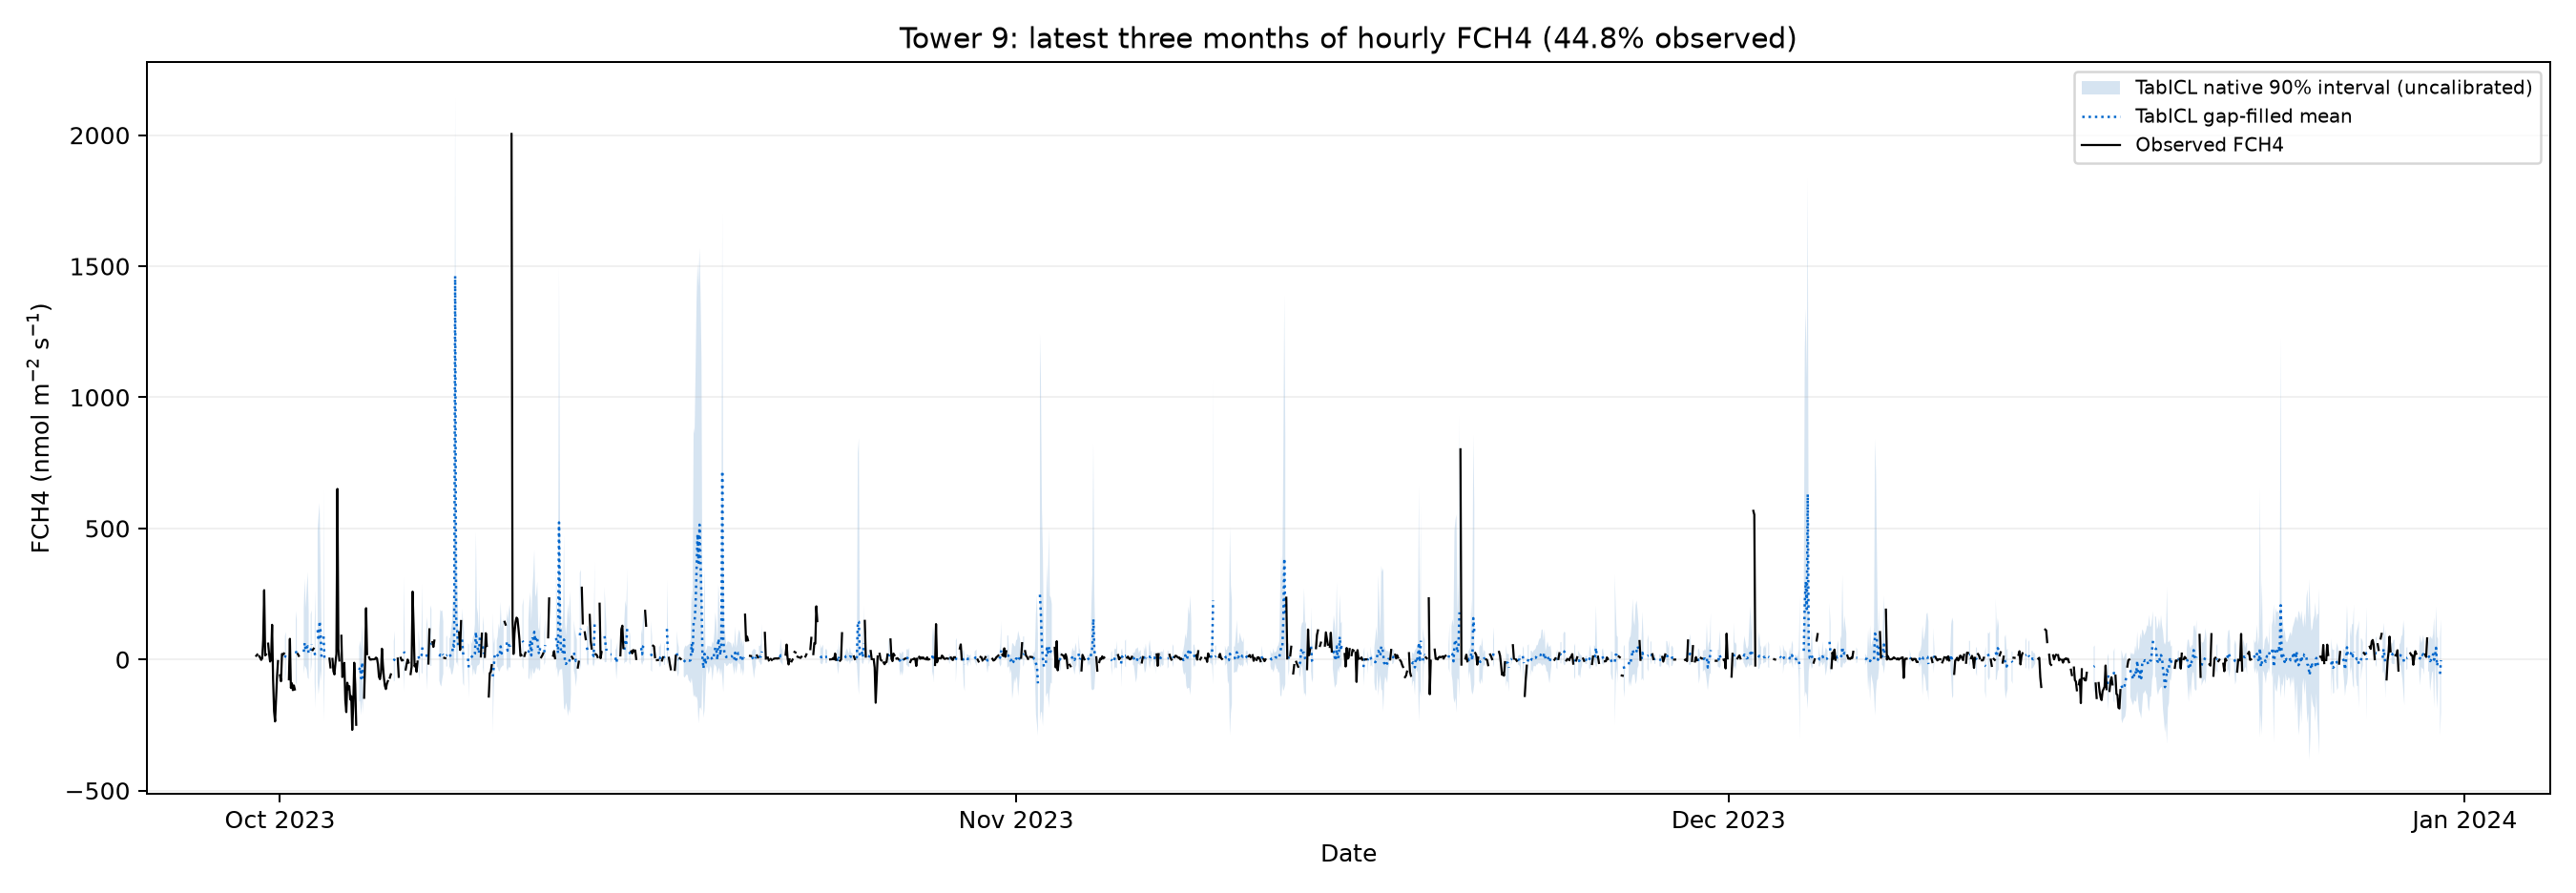
\includegraphics[width=\textwidth]{Figures/ch4_latest_tabicl_uq_hourly_T9_3month_example.png}
\caption{Three-month example of hourly FCH\textsubscript{4} reconstruction and
native uncertainty at T9. The figure shows QC-valid observations, the
TabICLv2 gap-filled mean and its uncalibrated native 90\% prediction interval
over the latest available three-month window, in which 44.8\% of the target
was observed. Corresponding T2 and T4 examples are provided in Appendix
Figure~\ref{fig:app_gf_tabicl_t2_t4}.}
\label{fig:gf_tabicl_hourly_examples}
\end{figure}

\FloatBarrier

Overall, TabICLv2 provides the strongest point reconstruction and is retained
as the gap-filling champion. Although calibrated coverage was close to the nominal target, the prediction 
intervals remained relatively wide, particularly at T9. Model identity and 
data-availability flags were therefore retained alongside the reconstructed 
FCH\textsubscript{4} series.

\FloatBarrier
